\documentclass[12pt, a4paper]{report}

% --- PACHETTI UTILIZZATI ---
\usepackage[utf8]{inputenc}
\usepackage[T1]{fontenc}
\usepackage[italian]{babel}
\usepackage{graphicx}
\usepackage{geometry}
\usepackage{hyperref}
\usepackage{array}
\usepackage{longtable}
\usepackage{booktabs}
\usepackage{caption}
\usepackage{xcolor}

% --- IMPOSTAZIONI DI PAGINA E STILE ---
\geometry{a4paper, top=3cm, bottom=3cm, left=2.5cm, right=2.5cm}
\hypersetup{
    colorlinks=true,
    linkcolor=blue,
    filecolor=magenta,      
    urlcolor=cyan,
    pdftitle={Documentazione Progetto DietiEstates25},
    pdfpagemode=FullScreen,
}

% --- DEFINIZIONE TABELLA COCKBURN ---
\newcolumntype{L}[1]{>{\raggedright\let\newline\\\arraybackslash\hspace{0pt}}m{#1}}
\newcolumntype{C}[1]{>{\centering\let\newline\\\arraybackslash\hspace{0pt}}m{#1}}
\newcolumntype{R}[1]{>{\raggedleft\let\newline\\\arraybackslash\hspace{0pt}}m{#1}}
\newcommand{\cockburn}[8]{
    \begin{center}
    \captionof{table}{Caso d'uso: #1}
    \begin{tabular}{|L{4cm}|L{11cm}|}
        \hline
        \textbf{Caso d'uso} & #1 \\
        \hline
        \textbf{Attori} & #2 \\
        \hline
        \textbf{Scopo} & #3 \\
        \hline
        \textbf{Precondizioni} & #4 \\
        \hline
        \textbf{Postcondizioni} & #5 \\
        \hline
        \textbf{Scenario Principale} & #6 \\
        \hline
        \textbf{Scenari Alternativi} & #7 \\
        \hline
        \textbf{Requisiti Speciali} & #8 \\
        \hline
    \end{tabular}
    \end{center}
}

% =====================================================================
% --- FRONTESPIZIO ---
% =====================================================================
\title{
    \vspace{2cm}
    
\includegraphics[width=0.4\textwidth]{images/logo.png} \\ % Aggiungi il logo Unina qui
    \textsc{\LARGE Università degli Studi di Napoli Federico II} \\
    \textsc{\Large Scuola Politecnica e delle Scienze di Base} \\[1.5cm]
    \rule{\linewidth}{0.5mm} \\[0.4cm]
    { \Large \bfseries Progetto di Ingegneria del Software \\ A.A. 2024/2025 \\[0.4cm] }
    \rule{\linewidth}{0.5mm} \\[1.5cm]
    \huge \textbf{DietiEstates25} \\
    \Large Documentazione di Progetto \\[2cm]
}
\author{
    \textbf{Gruppo:} INGSW2425\_XXX \\ % Sostituisci XXX con il tuo ID Gruppo
    \textbf{Componenti:} \\
    Nome Cognome - N86004374 \\
    Nome Cognome - N86004074 \\
    }
\date{\today}


% =====================================================================
% --- INIZIO DEL DOCUMENTO ---
% =====================================================================
\begin{document}

\maketitle
\tableofcontents
\newpage

% =====================================================================
% --- CAPITOLO 1: REQUISITI SOFTWARE ---
% =====================================================================
\chapter{Analisi dei Requisiti}
\label{cap:requisiti}
Questo capitolo definisce formalmente i requisiti del sistema DietiEstates25. L'analisi si concentra 
sull'identificazione degli attori che interagiscono con la piattaforma, sulla specifica dei vincoli 
qualitativi (requisiti non funzionali) e sulle regole di business (requisiti di dominio) che governano 
il comportamento dell'applicazione.

\section{Identificazione degli Attori del Sistema}

Sulla base dell'analisi delle esigenze operative, sono stati individuati cinque ruoli distinti, ciascuno 
caratterizzato da specifici privilegi e responsabilità all'interno della piattaforma.

\begin{itemize}
    \item \textbf{Admin (Amministratore di Sistema):} Rappresenta il livello gerarchico più alto. 
    L'Admin accede al sistema tramite credenziali predefinite e possiede il controllo globale sulla 
    piattaforma. Le sue responsabilità includono:
    \begin{itemize}
        \item Gestione completa degli annunci immobiliari e delle agenzie.
        \item Gestione e supervisione degli appuntamenti a livello globale.
        \item Creazione e gestione degli account privilegiati (Support, Manager, Agent) tramite il 
        sistema di inviti via email.
    \end{itemize}

    \item \textbf{Support (Operatore di Supporto):} È una figura operativa trasversale, concepita per 
    coadiuvare l'Amministratore. Possiede privilegi simili a quelli dell'Admin per garantire la continuità 
    operativa e la manutenzione dei contenuti, pur con lievi limitazioni sui permessi di gestione critica 
    del sistema.

    \item \textbf{Manager (Gestore di Agenzia):} È la figura responsabile dell'amministrazione di una 
    specifica agenzia immobiliare. Le sue competenze sono circoscritte al perimetro della propria agenzia:
    \begin{itemize}
        \item Creazione e configurazione della propria agenzia.
        \item Gestione del team di Agenti immobiliari afferenti alla sua struttura (inclusa la creazione 
        di nuovi account Agent tramite invito).
        \item Supervisione delle proprietà e degli appuntamenti associati alla propria agenzia.
    \end{itemize}

    \item \textbf{Agent (Agente Immobiliare):} Figura operativa focalizzata sulla vendita e l'affitto. 
    L'Agente ha autonomia nella creazione e gestione dei propri annunci immobiliari e si occupa di gestire 
    la propria agenda di appuntamenti con i clienti.

    \item \textbf{Customer (Cliente):} Rappresenta l'utente finale che fruisce dei servizi della piattaforma. 
    Il Customer può navigare liberamente tra le inserzioni, visualizzare i dettagli degli immobili e 
    richiedere appuntamenti. Ha inoltre accesso a un'area personale per monitorare lo stato delle proprie 
    richieste (es. confermate, in attesa o rifiutate).
\end{itemize}

\section{Requisiti Non Funzionali}

I requisiti non funzionali definiscono gli attributi di qualità del sistema, imponendo vincoli sulle 
modalità con cui le funzionalità devono essere erogate.

\begin{itemize}
    \item \textbf{Paradigma di Sviluppo:} Il sistema deve essere progettato e implementato seguendo 
    rigorosamente il paradigma Orientato agli Oggetti (Object-Oriented), garantendo modularità e 
    manutenibilità del codice.

    \item \textbf{Usabilità e Interfaccia:} Il sistema deve presentare un'interfaccia utente (UI) 
    intuitiva, conforme ai principi di Human-Centered Design, che garantisca una chiara gerarchia 
    visiva delle informazioni relative agli immobili.

    \item \textbf{Prestazioni ed Efficienza:} Il motore di ricerca deve garantire tempi di risposta 
    inferiori ai 2 secondi per il 99\% delle query effettuate, assicurando un'esperienza utente fluida 
    anche con elevati volumi di dati.

    \item \textbf{Sicurezza:} Il sistema deve implementare protocolli sicuri per l'archiviazione e la 
    gestione delle credenziali degli utenti, proteggendo i dati sensibili da accessi non autorizzati.

    \item \textbf{Accessibilità e Curva di Apprendimento:}
    \begin{itemize}
        \item Per i Customer: L'utilizzo delle funzionalità core (ricerca, prenotazione) deve essere 
        immediato e non richiedere alcuna formazione pregressa ("Walk-up-and-use").
        \item Per gli Operatori (Admin, Manager, Agent): L'interfaccia di gestione deve permettere di 
        raggiungere la piena operatività con un training minimo (inferiore ai 30 minuti), minimizzando 
        il tasso di errore operatore durante l'uso prolungato.
    \end{itemize}

    \item \textbf{Affidabilità:} Il sistema deve garantire un Service Level Agreement (SLA) con un 
    tempo di disponibilità (uptime) del 99\% su base mensile.
\end{itemize}

\section{Requisiti di Dominio}

I requisiti di dominio specificano vincoli derivanti dal contesto operativo e normativo del settore 
immobiliare in cui il sistema opera, nonché le regole di business fondamentali per la gestione degli 
utenti e dei servizi.

\begin{itemize}
    \item \textbf{Onboarding e Registrazione Privilegiata:} Al fine di garantire la sicurezza e il 
    controllo degli accessi, la registrazione per i ruoli operativi (Agent, Manager, Support) non deve 
    essere accessibile pubblicamente. Il sistema deve prevedere un meccanismo di invito tramite email: 
    l'amministratore o il gestore generano un link univoco che, una volta inviato all'utente, consente 
    la registrazione diretta con il ruolo specifico pre-assegnato.

    \item \textbf{Gestione Notifiche e Appuntamenti:} Il sistema deve garantire un flusso di comunicazione 
    proattivo verso gli utenti. È richiesto l'invio automatico di aggiornamenti (tramite email o notifiche 
    interne) relativi allo stato delle richieste di appuntamento (es. in attesa, confermato, rifiutato), 
    permettendo a clienti e agenti di monitorare l'evoluzione delle prenotazioni in tempo reale.

    \item \textbf{Gestione Inserzioni:} La facoltà di caricare e pubblicare nuovi annunci immobiliari 
    è riservata esclusivamente ai ruoli operativi (Admin, Support, Manager, Agent). L'utente con ruolo 
    Customer non dispone dei privilegi di scrittura per le inserzioni.

    \item \textbf{Gestione Agenti e Assegnazione:} Il sistema deve prevedere una funzionalità dedicata 
    per gli amministratori (Admin) e il supporto tecnico (Support) che permetta di visualizzare l'elenco 
    degli agenti immobiliari non ancora affiliati ad alcuna agenzia. Tale funzionalità deve consentire 
    l'assegnazione operativa di questi agenti a una specifica agenzia esistente.

    \item \textbf{Conformità Normativa:} In fase di creazione dell'annuncio, il sistema deve validare 
    la presenza di informazioni obbligatorie secondo la normativa vigente, tra cui: classe energetica 
    (D.Lgs. 192/2005), metratura commerciale, numero di vani e prezzo.

    \item \textbf{Supporto Decisionale (Meteo e Mappa):} Il sistema deve integrare servizi di terze 
    parti per arricchire l'esperienza di prenotazione:
    \begin{itemize}
        \item Una mappa interattiva per la geolocalizzazione precisa dell'immobile.
        \item Un widget per le previsioni meteo in tempo reale, per supportare l'utente nella scelta 
        ottimale della data per la visita in loco.
    \end{itemize}

    \item \textbf{Categorizzazione e Ricerca Flessibile:} Il sistema deve classificare primariamente 
    gli immobili in base alla tipologia contrattuale (Vendita o Affitto). Sebbene non sia imposta una 
    tassonomia rigida per la tipologia edilizia (es. menu a tendina bloccati), il sistema deve permettere 
    il filtraggio e la ricerca avanzata basata sulle caratteristiche descrittive inserite, garantendo 
    flessibilità nel reperimento dell'immobile desiderato.
\end{itemize}

\section{Glossario}
\begin{description}
    \item[Agenzia Immobiliare] Entità che gestisce un insieme di agenti e inserzioni immobiliari.
    \item[Agente Immobiliare] Utente autorizzato a inserire, modificare e gestire le inserzioni di immobili per conto di un'agenzia.
    \item[Utente/Cliente] Utente finale che cerca, visualizza immobili, prenota visite e fa offerte.
    \item[Inserzione] Annuncio di un immobile in vendita o in affitto, completo di dettagli.
    \item[Amministratore] Utente gestore dell'agenzia con privilegi elevati.
    \item[UML (Unified Modeling Language)] Standard industriale di modellazione visuale. Fornisce un vocabolario grafico unificato per specificare, costruire e documentare l'architettura di un sistema software attraverso diverse tipologie di diagrammi (strutturali e comportamentali).
    \item[Mockup] Prototipo visivo statico dell'interfaccia utente (UI). Viene utilizzato nelle fasi preliminari per definire il layout grafico e validare l'esperienza utente (UX) prima dell'effettiva implementazione del codice.
    \item[Casi d’uso (Use Case)] Descrizione funzionale del comportamento del sistema in risposta a una richiesta esterna. Definiscono i requisiti funzionali narrando come il sistema interagisce con l'ambiente per raggiungere uno specifico obiettivo di business.
    \item[Tabelle di Cockburn] Formalismo strutturato per la documentazione dettagliata dei casi d'uso. Scompongono l'interazione in uno schema rigoroso che include il flusso principale degli eventi, le precondizioni, le garanzie di successo e la gestione delle eccezioni (scenari alternativi).
    \item[Attore] Qualsiasi entità esterna al perimetro del sistema (utente umano, dispositivo hardware o software di terze parti) che interagisce con esso scambiando informazioni o avviando processi.
    \item[Personas] Archetipi di utenti fittizi, costruiti su dati reali, che rappresentano i diversi segmenti di pubblico target. Sono uno strumento fondamentale di design per focalizzare lo sviluppo sulle reali necessità e comportamenti degli utenti finali.
    \item[Use Case Diagram] Diagramma UML che offre una visione di alto livello delle funzionalità del sistema. Definisce il confine del progetto (scope), illustrando le relazioni tra gli attori esterni e i casi d'uso supportati.
    \item[Sequence Diagram] Diagramma UML di interazione che descrive la dinamica temporale di un processo. Mappa l'ordine cronologico dei messaggi scambiati tra i vari oggetti o componenti del sistema per completare una specifica operazione.
    \item[API (Application Programming Interface)] Insieme di protocolli e strumenti che permette l'interoperabilità tra diverse applicazioni software. Funge da contratto di interfaccia, consentendo lo scambio di dati e funzionalità astraendo dalla complessità dell'implementazione sottostante.
    \item[Front-end] Il livello di presentazione dell'architettura software. Comprende l'interfaccia utente e la logica eseguita lato client (es. nel browser), gestendo direttamente l'interazione visiva con l'utente.
    \item[Back-end] Il livello di accesso ai dati e logica di business. Risiede sul server e gestisce l'elaborazione delle richieste, la sicurezza, le regole applicative e la persistenza delle informazioni nel database, rimanendo invisibile all'utente finale.
\end{description}


\chapter{Individuazione e Caratterizzazione degli Utenti (Personas)}
\label{cap:personas}
In questa sezione vengono presentate le \textit{personas} individuate per il progetto \textbf{DietiEstates25}. Le \textit{personas} sono rappresentazioni fittizie di utenti tipici che utilizzano il sistema, create per comprendere meglio le esigenze, i comportamenti e gli obiettivi degli utenti finali. Queste rappresentazioni aiutano il team di sviluppo a mantenere un focus centrato sull'utente durante tutto il processo di progettazione e sviluppo del software.

 \subsection{Giulia Ricci - Il Cliente in Cerca della Prima Casa}

  \begin{figure}[H]
     \centering
     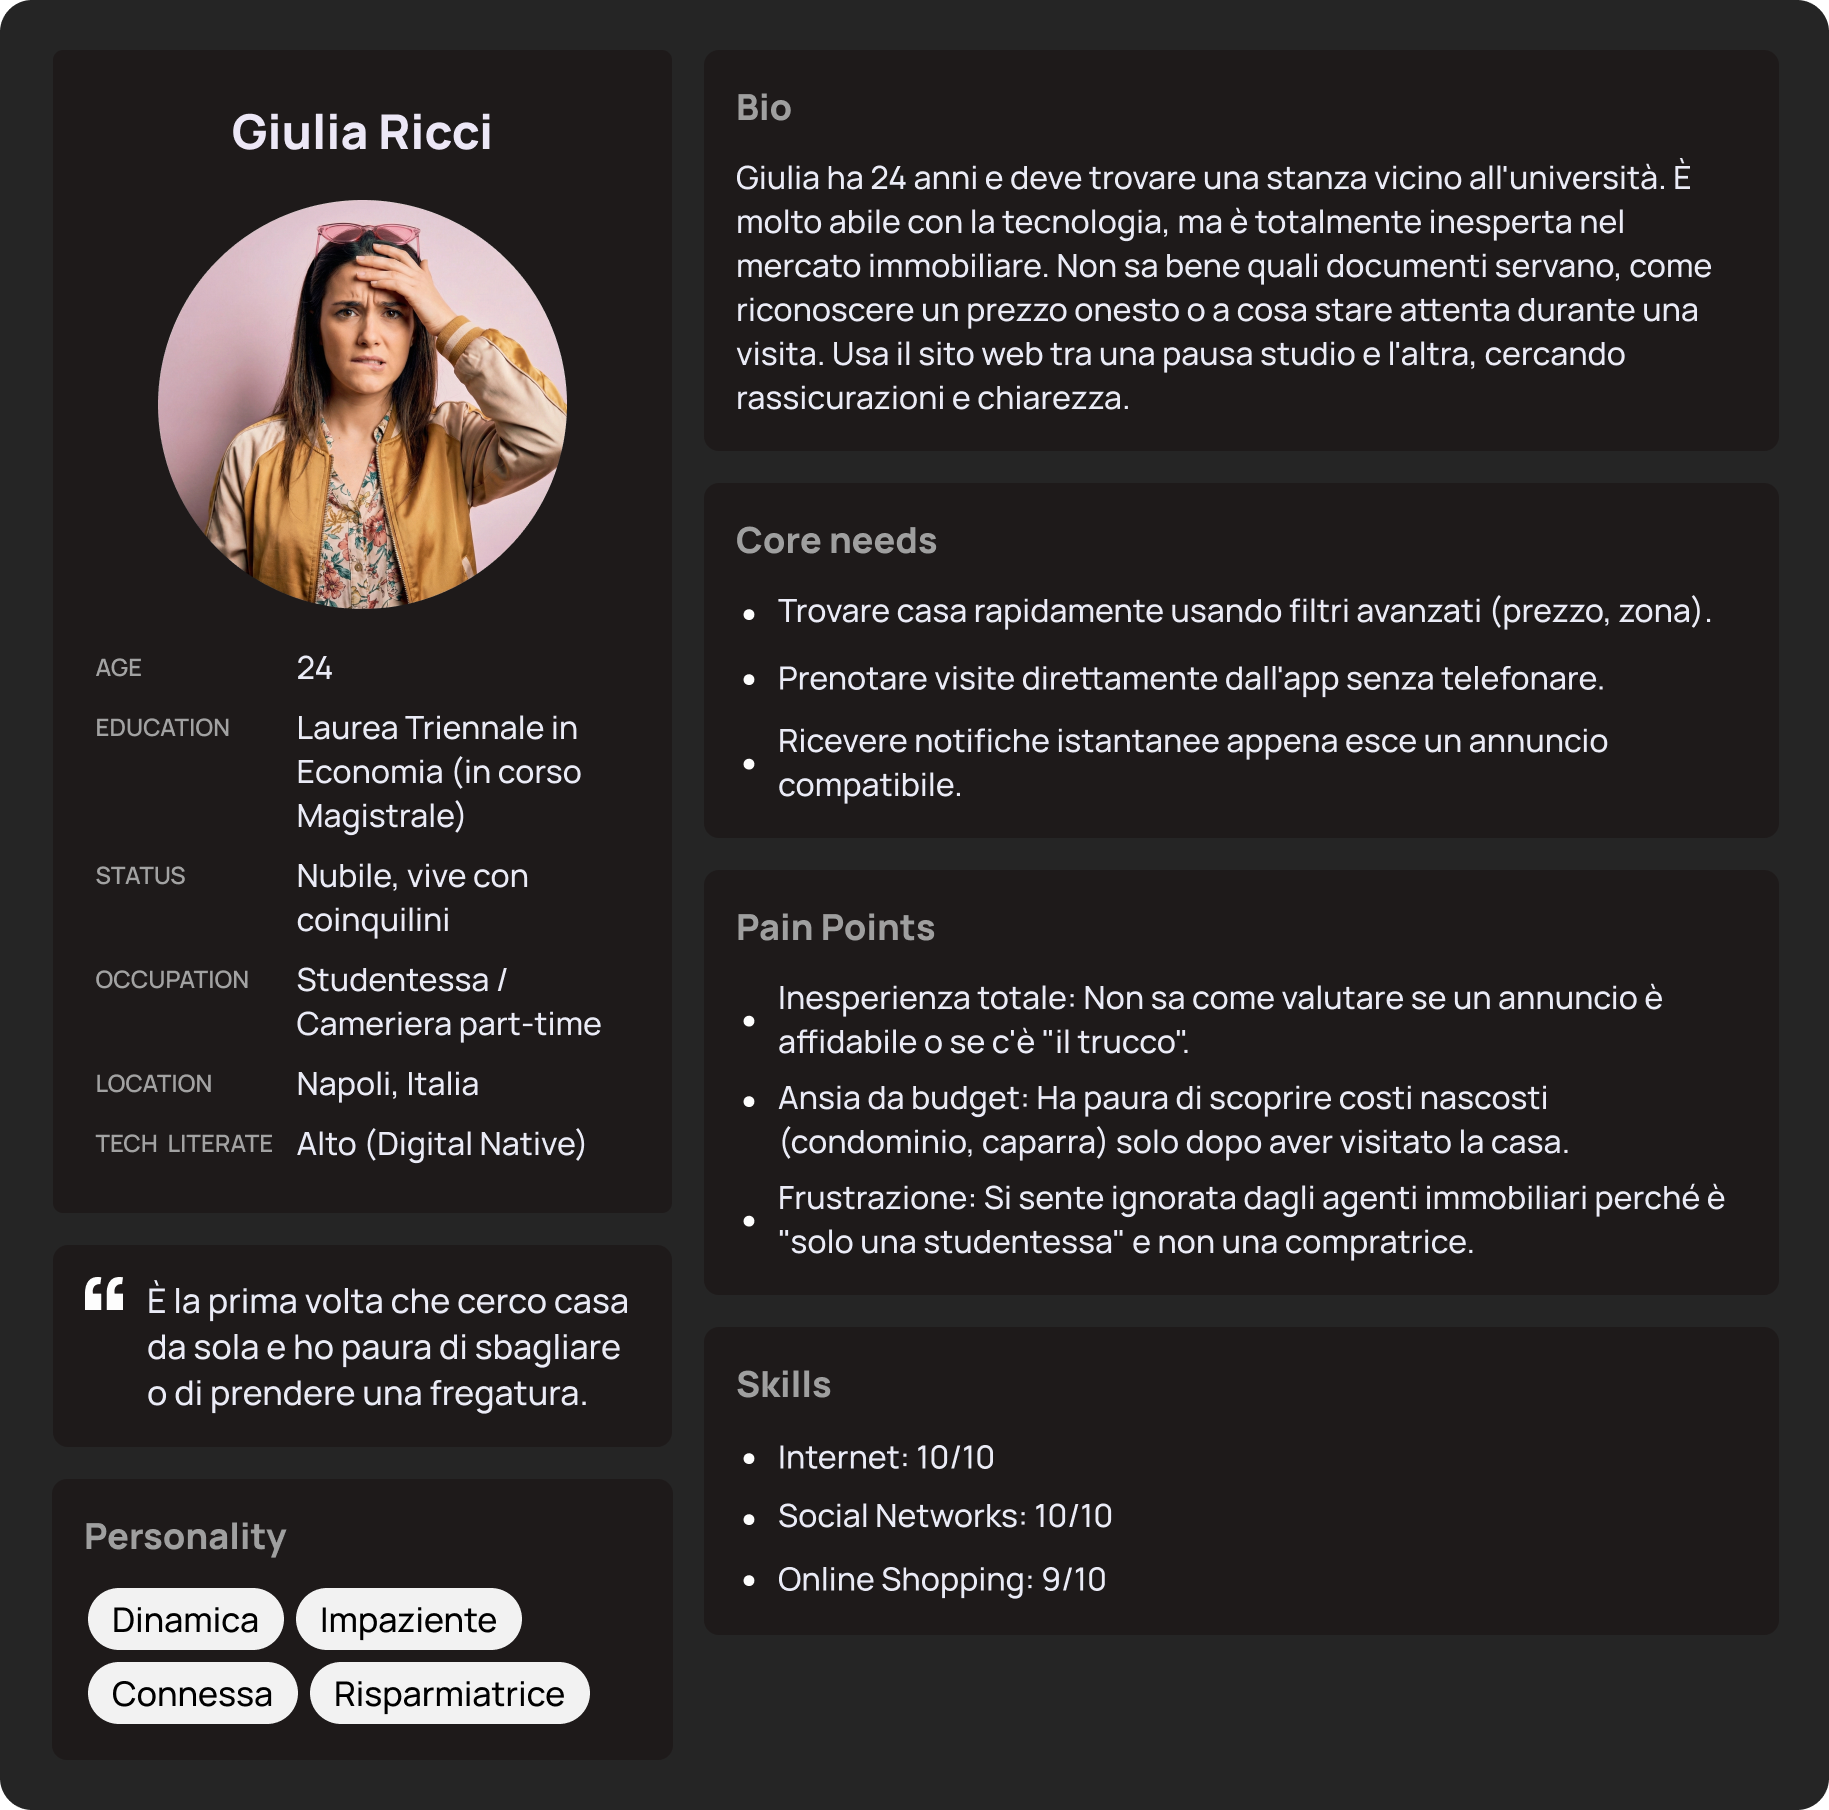
\includegraphics[width=0.8\textwidth]{images/Giulia.png}
     \caption{Personas Studentessa Universitaria - Giulia Ricci}
     \label{fig:P1}
 \end{figure}

   \subsection{Antonio Bianchi  - Utente Poco Esperto di Tecnologia}

  \begin{figure}[H]
     \centering
     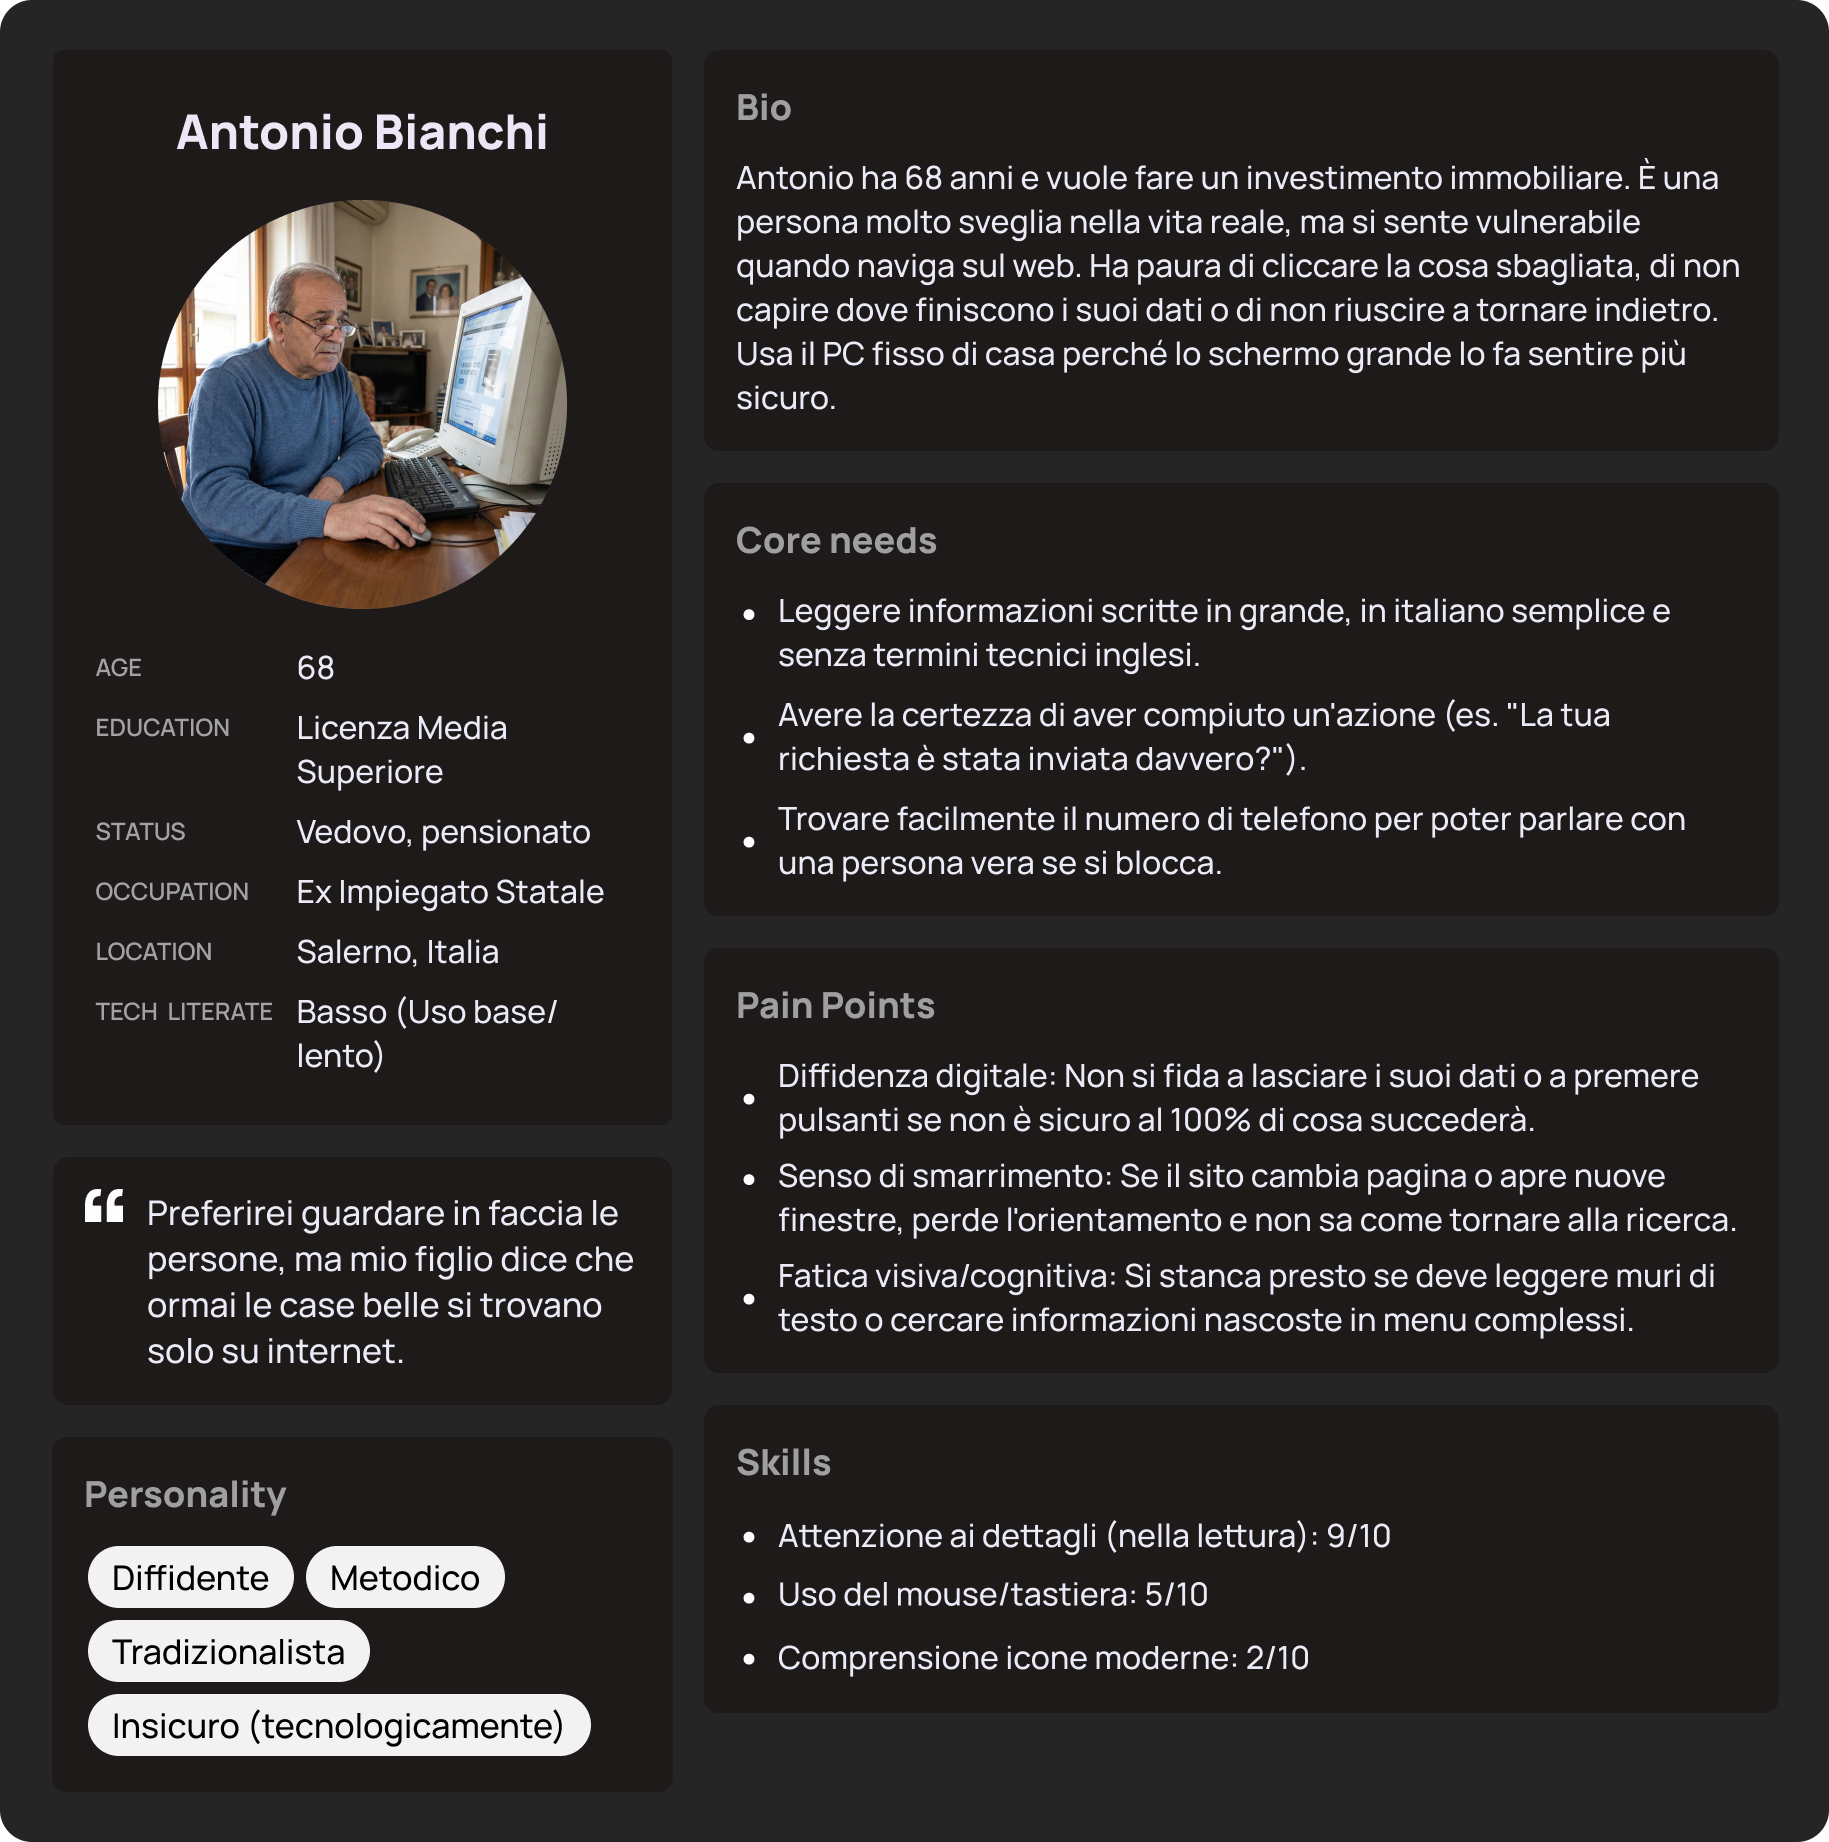
\includegraphics[width=0.8\textwidth]{images/Antonio.png}
     \caption{Personas Utente Poco Esperto di Tecnologia - Antonio Bianchi}
     \label{fig:P2}
 \end{figure}
 
  \subsection{Marco Esposito  - Agente Immobiliare}

  \begin{figure}[H]
     \centering
     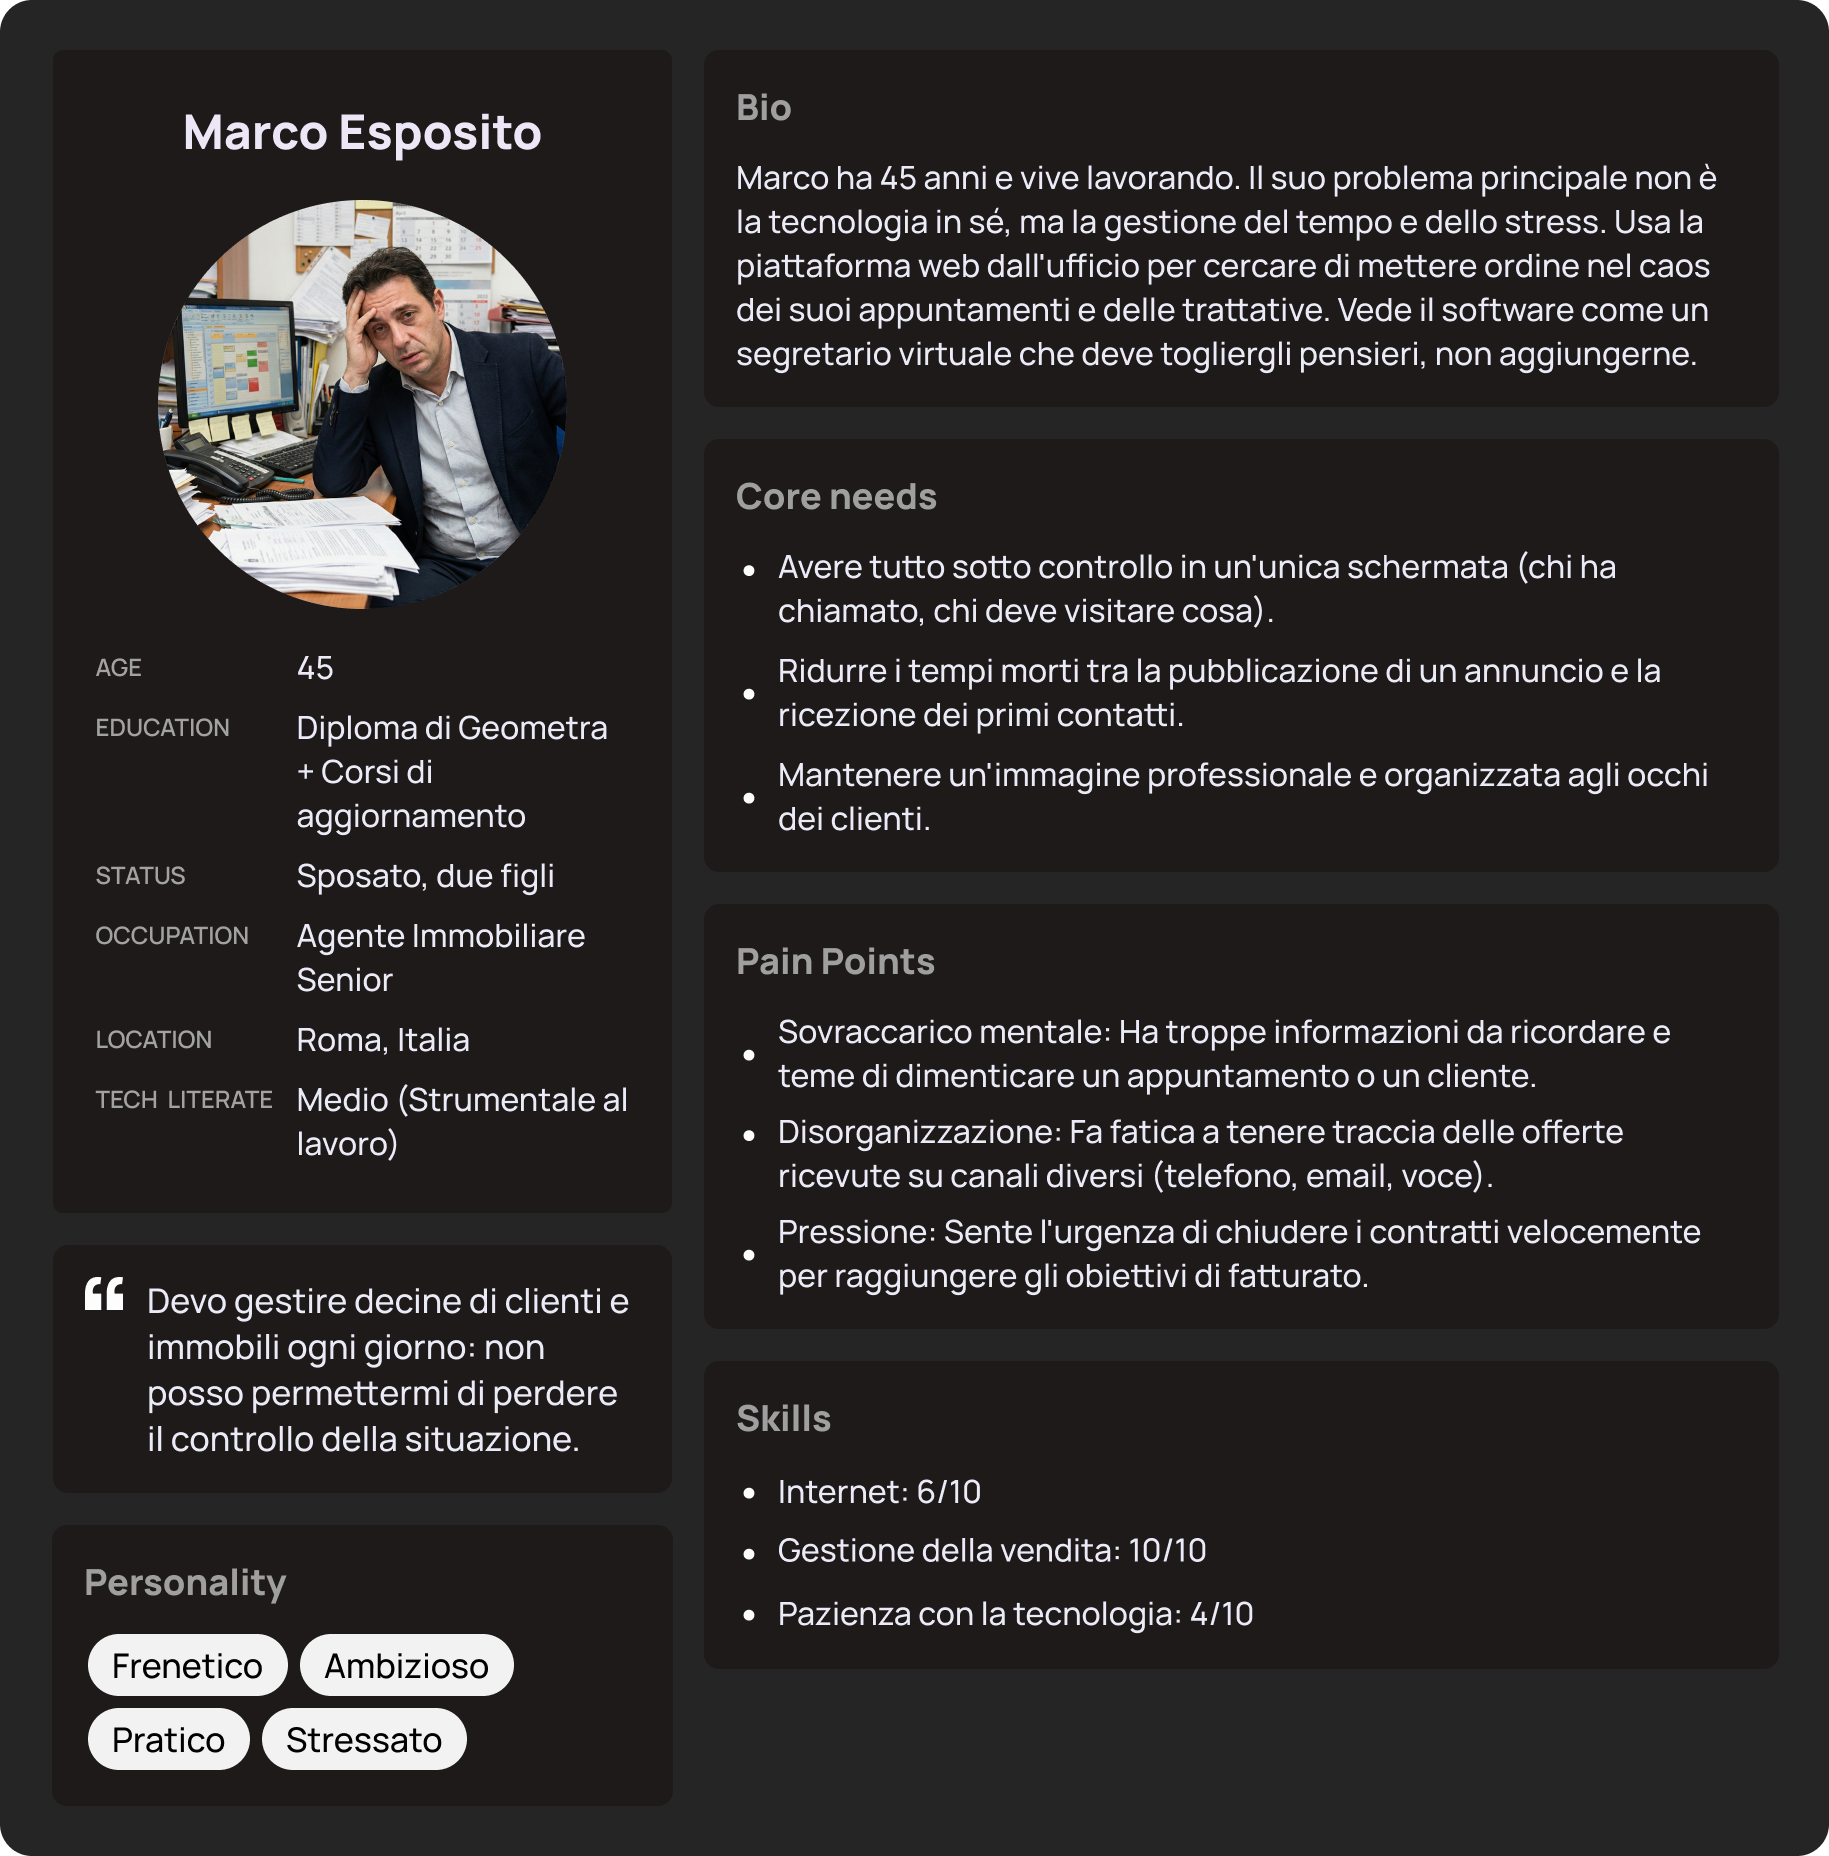
\includegraphics[width=0.8\textwidth]{images/Marco.png}
     \caption{Personas Agente Immobiliare - Marco Esposito}
     \label{fig:P3}
 \end{figure}

   \subsection{Roberto De Luca  - Manager di Agenzia Immobiliare}

  \begin{figure}[H]
     \centering
     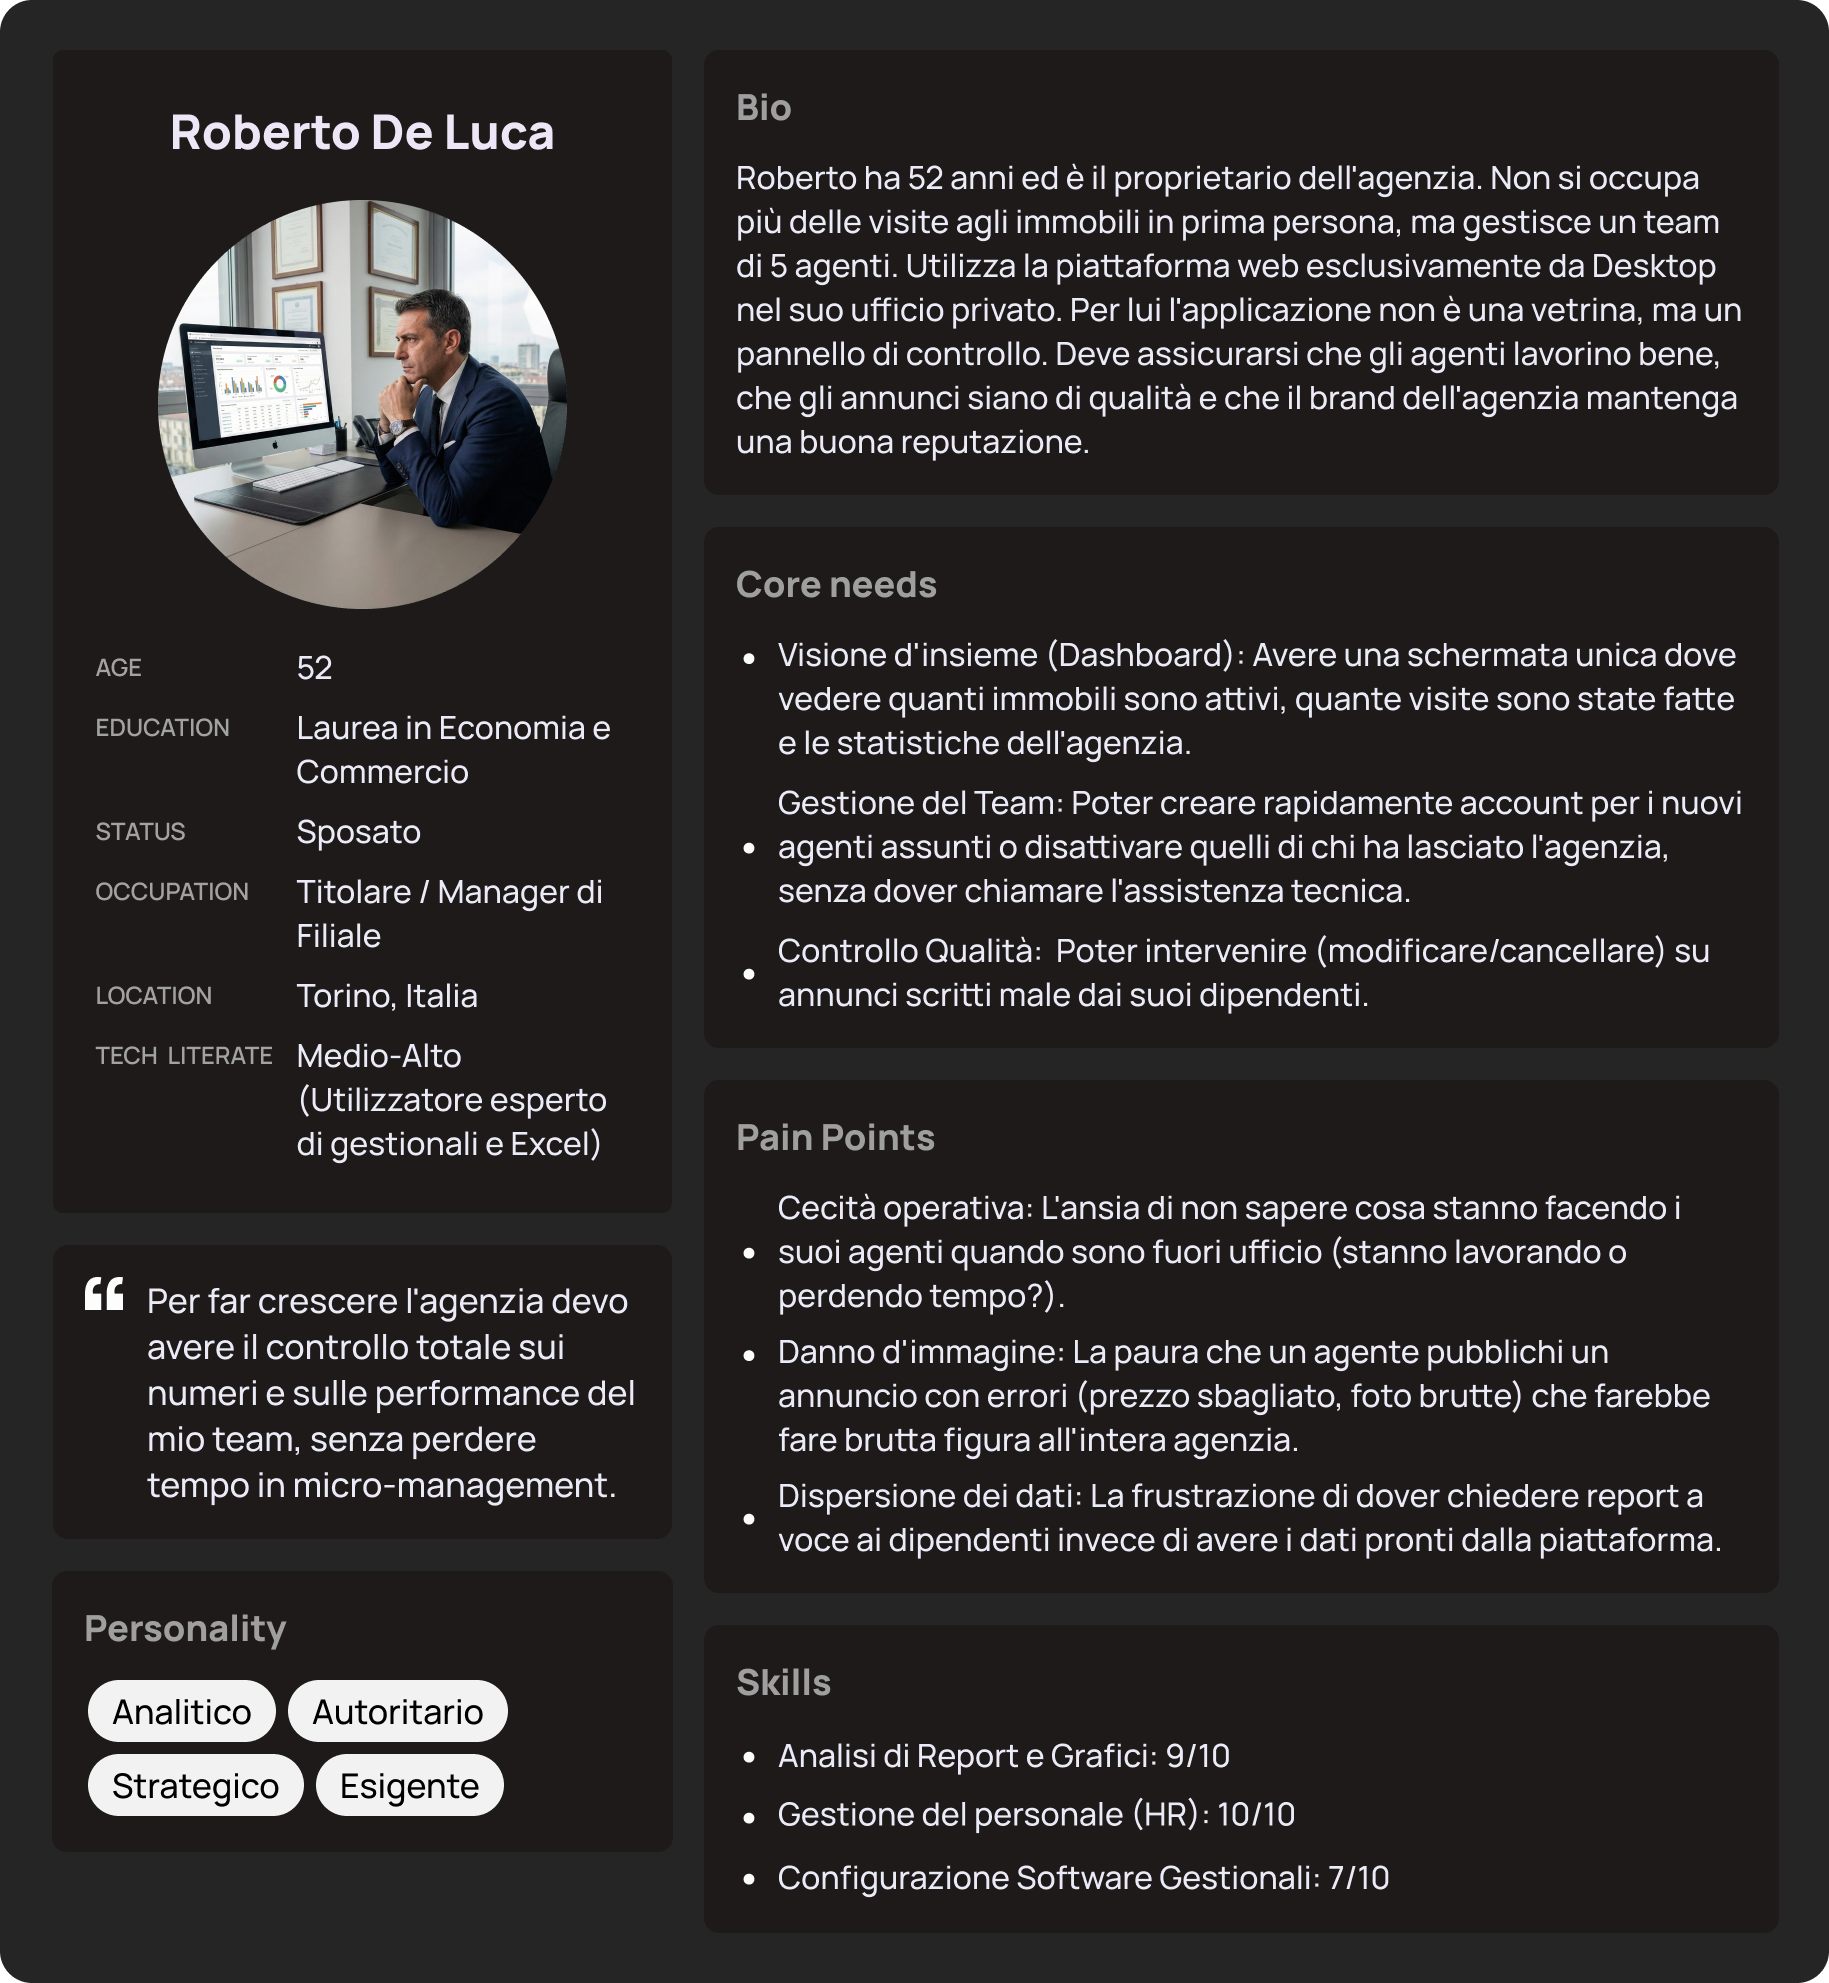
\includegraphics[width=0.8\textwidth]{images/Roberto.png}
     \caption{Personas Manager di Agenzia Immobiliare - Roberto De Luca}
     \label{fig:P4}
 \end{figure}
 

%% =====================================================================
% --- CAPITOLO 3: ARTEFATTI E PROCESSO DI SVILUPPO ---
% =====================================================================
\chapter{Artefatti e Processo di Sviluppo}
\label{cap:artefatti}
% Riferimento Traccia: "Output: Artefatti Software e documentazione del processo di sviluppo"

Questo capitolo descrive gli artefatti tecnici prodotti e i processi utilizzati per la gestione del codice sorgente, la qualità e il deployment.

\section{Strumenti di Versioning: GitHub}

Per la gestione del codice sorgente e il versionamento del progetto, il team ha scelto di utilizzare GitHub. GitHub è una piattaforma di hosting basata sul sistema di controllo versione distribuito Git. Essa non si limita a fungere da archivio remoto per il codice, ma offre un ecosistema completo per il social coding, integrando strumenti per la gestione delle issue, la revisione del codice (Code Review) e l'automazione dei flussi di lavoro (CI/CD). La scelta di GitHub ha permesso di centralizzare lo sviluppo, garantendo un punto di riferimento unico e sincronizzato per tutti i membri del gruppo.

\subsection{Vantaggi dell'adozione di GitHub}
L'utilizzo di GitHub come strumento di versioning ha apportato benefici tangibili al flusso di lavoro del team, in particolare:

\begin{itemize}
    \item \textbf{Collaborazione facilitata:} GitHub ha permesso al team di lavorare in parallelo su diverse 
    funzionalità senza conflitti bloccanti. Attraverso l'uso dei branch (ramificazioni), ogni sviluppatore 
    ha potuto isolare il proprio ambiente di sviluppo per lavorare su feature specifiche o bugfix. 
    L'integrazione delle modifiche nel ramo principale (main/master) è avvenuta tramite Pull Requests (PR), 
    un meccanismo che ha facilitato la discussione sulle modifiche e la Code Review prima del merge definitivo, 
    migliorando la qualità complessiva del codice.

    \item \textbf{Tracciamento delle modifiche:} La piattaforma offre una visibilità granulare su ogni singola 
    modifica apportata al progetto. Grazie alla cronologia dei commit, è possibile identificare esattamente 
    "chi ha fatto cosa e quando". Questo livello di trasparenza è fondamentale non solo per monitorare 
    l'avanzamento dei lavori, ma anche per il debugging, permettendo di risalire rapidamente all'origine 
    di eventuali errori introdotti nel codice.

    \item \textbf{Ritorno a versioni precedenti (Rollback):} Uno dei vantaggi critici di un sistema di 
    versioning robusto è la possibilità di viaggiare nel tempo all'interno del progetto. In caso di 
    aggiornamenti che introducono regressioni o errori critici, GitHub permette di ripristinare rapidamente 
    lo stato del software a una versione precedente, stabile e funzionante. Questo garantisce una 
    "rete di sicurezza" continua durante tutto il ciclo di sviluppo.

    \item \textbf{Backup e sicurezza:} Essendo un sistema distribuito, il codice risiede sia localmente 
    sulle macchine degli sviluppatori sia sul repository remoto nel cloud di GitHub. Questa ridondanza 
    funge da backup automatico: anche in caso di guasto hardware di un computer locale, il lavoro non 
    viene perso ed è immediatamente recuperabile dal server remoto. Inoltre, GitHub permette di gestire 
    i permessi di accesso, proteggendo il ramo principale da modifiche non autorizzate o accidentali.
\end{itemize}

\section{Report di Qualità del Codice (SonarQube)}
La qualità del software non si misura solo attraverso il corretto funzionamento delle funzionalità, 
ma anche tramite la struttura interna del codice sorgente. Adottare standard elevati di Clean Code 
è essenziale per garantire la sostenibilità del progetto: un codice pulito riduce il debito tecnico, 
accelera l'inserimento di nuovi sviluppatori e semplifica le future fasi di manutenzione ed evoluzione, 
minimizzando il rischio di regressioni.

\subsection{Analisi Statica con SonarQube}
Per oggettivare la qualità del software prodotto, il team ha integrato nel flusso di sviluppo SonarQube, una piattaforma di analisi statica automatizzata. Questo strumento esegue una scansione continua del codice, evidenziando le aree critiche e fornendo metriche precise per guidare le attività di refactoring.

L'analisi si è focalizzata sulle seguenti metriche chiave:

\begin{itemize}
    \item \textbf{Bugs (Affidabilità):} Identificano errori di logica o di programmazione che porteranno quasi sicuramente a un malfunzionamento o a un crash dell'applicazione in fase di esecuzione. La loro risoluzione ha priorità massima per garantire la stabilità del sistema.

    \item \textbf{Vulnerabilità (Sicurezza):} Segnalano punti deboli nel codice che potrebbero essere sfruttati da attacchi esterni (come Injection o esposizione di dati sensibili). Monitorare questo indice è cruciale per garantire la sicurezza dei dati e l'integrità del sistema.

    \item \textbf{Code Smells (Manutenibilità):} Non si tratta di errori bloccanti, ma di violazioni delle buone pratiche di programmazione (es. classi troppo grandi, complessità ciclomatica elevata, nomi di variabili poco chiari). Se trascurati, rendono il codice difficile da leggere e modificare, aumentando i costi di manutenzione futuri.

    \item \textbf{Duplicazioni (Ridondanza):} Rilevano blocchi di codice identici ripetuti in più punti (violazione del principio DRY - Don't Repeat Yourself). Le duplicazioni sono pericolose perché richiedono che ogni modifica venga replicata manualmente in tutti i punti, aumentando il rischio di errore umano.
\end{itemize}

\textit{[Placeholder per screenshot SonarQube (Quality Gate, Bugs, Vulnerabilities, Code Smells).]}

\section{Containerizzazione (Dockerfile)}
% Riferimento Traccia: "Codice Sorgente sviluppato, comprensivo di eventuale Dockerfile."
% Riferimenti Slide: 24 - Virtualizzazione e Cloud.pdf
Come richiesto, il backend è stato containerizzato tramite \textbf{Docker} per garantire portabilità e riproducibilità. Di seguito è riportato il \texttt{Dockerfile} utilizzato per il backend Express:

\begin{lstlisting}[language=bash, caption={Dockerfile per il backend Node.js/Express}]
# Stage 1: Build
FROM node:18-alpine AS builder
WORKDIR /usr/src/app

# Copia package.json e installa le dipendenze
COPY package*.json ./
RUN npm install

# Copia il resto del codice sorgente
COPY . .

# Compila il codice TypeScript
RUN npm run build

# Stage 2: Produzione
FROM node:18-alpine
WORKDIR /usr/src/app

# Copia solo i file necessari dalla build precedente
COPY --from=builder /usr/src/app/package*.json ./
COPY --from=builder /usr/src/app/dist ./dist

# Installa solo le dipendenze di produzione
RUN npm ci --only=production

# Esponi la porta
EXPOSE 3000

# Comando di avvio
CMD [ "node", "dist/index.js" ]
\end{lstlisting}

\section{File di Build Automatica}
% Riferimento Traccia: "File di build automatica"
La build automatica è gestita tramite gli script NPM definiti in \texttt{package.json} e orchestrati dal \texttt{Dockerfile}. Lo script \texttt{npm run build} (che esegue \texttt{tsc}) compila il codice TypeScript in JavaScript.

Il deployment è automatizzato tramite \texttt{docker-compose.yml}, che orchestra l'avvio del container dell'applicazione e del database.



\end{document}